\chapter{Przedstawienie zastosowanych narzędzi}\label{chap:przedstawienie_zastosowanych_narzędzi}

\section{Język programowania}
Obecnie, Python, język programowania wysokiego poziomu ogólnego przeznaczenia, wprowadzony w 1991 roku przez Guido van Rossum’a \cite{Python}, dominuje w dziedzinie sztucznej inteligencji. Charakteryzuje się on prostą składnią, która ułatwia naukę i stosowanie w praktyce, co czyni go szczególnie popularnym wśród inżynierów danych. Python jest ceniony za wsparcie licznych bibliotek specjalizujących się w przetwarzaniu danych i uczeniu maszynowym, jak również za otwartoźródłowy charakter, co umożliwia szeroką współpracę w społeczności naukowej. W pracy przedstawione zostały modele wykorzystujące język Python w połączeniu z biblioteką PyTorch \cite{paszke2019}, która jest rozwijana na bazie Torch i umożliwia efektywne budowanie oraz trenowanie modeli głębokiego uczenia z użyciem procesora graficznego.

\section{Platforma obliczeniowa}
W celu uruchomienia analizowanych metod neuronowych wizyjnych algorytmów percepcji głębi, wykorzystano platformę obliczeniową Google Colab. Jest to platforma sieciowa, która umożliwia uruchamianie skryptów w języku Python bezpośrednio w przeglądarce, co jest szczególnie korzystne w kontekście prac badawczych i edukacyjnych\footnote{\href{https://colab.google/}{https://colab.google/}}. Platforma ta opiera się na technologii Jupyter Notebook, co umożliwia interaktywne programowanie i wizualizację danych\footnote{\href{https://jupyter.org/}{https://jupyter.org/}}.

Google Colab oferuje dostęp do mocnych zasobów obliczeniowych, w tym do procesorów graficznych (GPU) i jednostek przetwarzania tensorów (TPU), które są kluczowe przy trenowaniu skomplikowanych modeli głębokiego uczenia. Użytkownicy mogą łatwo skalować użycie zasobów w zależności od potrzeb danego algorytmu, co znacząco redukuje czas i koszt przetwarzania. Dostępność tych zasobów przez platformę internetową umożliwia również łatwe udostępnianie wyników i współpracę w ramach zespołów rozproszonych geograficznie.

W kontekście przeprowadzonej analizy, Google Colab okazał się być nieocenionym narzędziem, które pozwoliło na efektywne wykonanie i analizę algorytmów percepcji głębi. Możliwość wyświetlania wyników bezpośrednio w przeglądarce internetowej znacząco ułatwiła proces badawczy i pozwoliła na dynamiczne dopasowanie parametrów modelu w odpowiedzi na obserwowane wyniki.

\section{Zestawy danych}
Niewątpliwie kluczową rolę w procesie analizy porównawczej algorytmów percepcji głębi odgrywają odpowiednio dobrane zestawy danych. Wiele metod jest testowanych przez ich twórców na zbiorach tożsamych do tych na których były uczone. Powoduje to brak poprawnej oceny zdolności do generalizacji danego algorytmu na niewidzianych podczas uczenia scenach. W celu uniknięcia tego typu błędów, w niniejszej pracy do analizy algorytmów wykorzystano zestawy danych, które są dostępne publicznie, jednak nie zostały wykorzystane w trenowaniu ani testowaniu żadnej analizowanej metody.

Ponadto każda z metod została zweryfikowana na autorskim zestawie danych. Został on przygotowany na potrzeby niniejszej pracy za pomocą technologii LIDAR stanowiącej wyposażenie urządzenia iPhone 15 Pro \cite{chase2022apple}. Zastosowany w rzeczonym urządzeniu skaner emituje matrycę zawierającą 8x8 punktów która jest podzielona na siatki 3x3 co daje łącznie 576 punktów. Maksymalny zasięg tego skanera to 5 metrów. Fotografie i skany zostały wykonane w otwartych przestrzeniach we Wrocławskim Ogrodzie Zoologicznym. Obrazy RGB wraz z odpowiadającymi im mapami głębi pochodzącymi z autorskiego zestawu są dostępne w załączniku do pracy.
\begin{figure}[H]
    \centering
    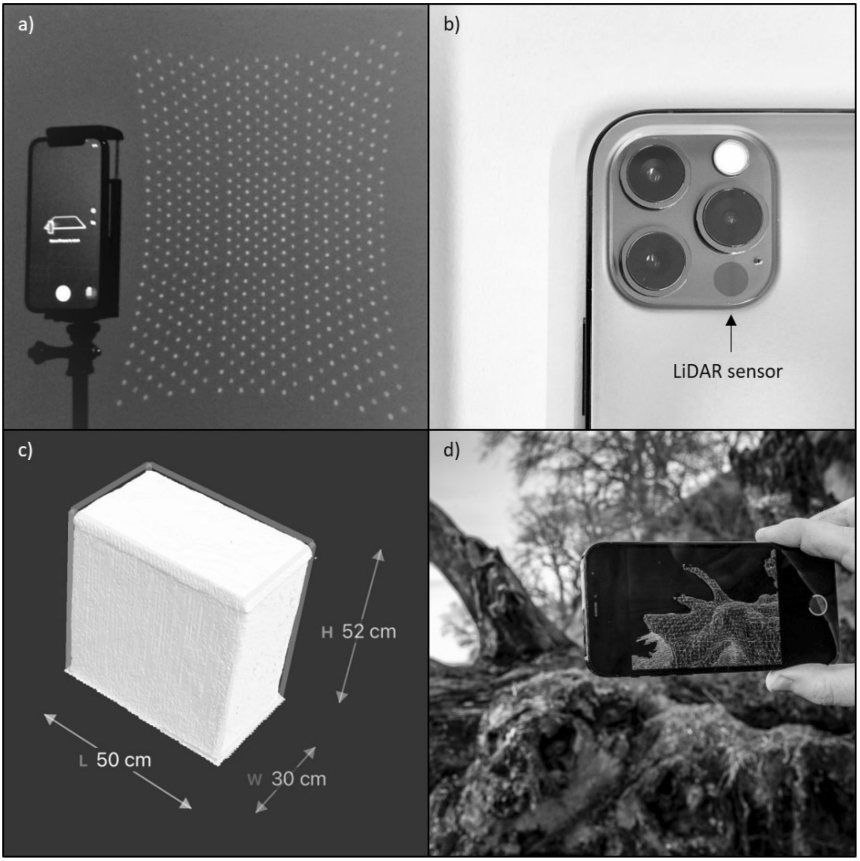
\includegraphics[width=0.55\textwidth]{45.jpg}
    \caption{a) emitowana matryca punktów b) umiejscowienie skanera w urządzeniu c) przykładowy model 3D wykonany przy użycciu skanera d) przykład implementacji w oprogramowaniu. Źródło: \cite{luetzenburg2021evaluation}}
    \label{fig:iphone-lidar}
\end{figure}

\section{Narzędzia do analizy i wizualizacji}
Tutaj będzie m.in. informacja o użyciu biblioteki Matplotlib i OpenCV.
